%%%% fatec-article.tex, 2024/03/10

%% Classe de documento
\documentclass[
  a4paper,%% Tamanho de papel: a4paper, letterpaper (^), etc.
  12pt,%% Tamanho de fonte: 10pt (^), 11pt, 12pt, etc.
  english,%% Idioma secundário (penúltimo) (>)
  brazilian,%% Idioma primário (último) (>)
]{article}

%% Pacotes utilizados
\usepackage[]{fatec-article}
\usepackage{float}
\usepackage{algorithm}
\usepackage{algpseudocode}
\usepackage{amsmath}

\Author{1}{Name={ Fagundes. L \\ Freitas. A \\ Freitas. V}}

\Author{2}{Name={\{ lucas.fagundes3@fatec.sp.gov.br \}\\ \{ amanda.freitas14@fatec.sp.gov.br \} \\ \{ valeria.freitas@fatec.sp.gov.br \}}}

%% Definição das palavras-chaves/keywords
\Keyword{1}{Citrus reticulata}{Citrus reticulata}
\Keyword{2}{Deficiência nutricional}{Nutritional deficiency}
\Keyword{3}{Visão computacional}{Computer Vision}
\Keyword{4}{Manganês}{Manganese}
\Keyword{5}{Cobre}{Copper}

%%%% Resumo no idioma primário (brazilian)
\begin{Abstract}[brazilian]%% Idioma (brazilian ou english)
  Este artigo tem como objetivo alinhar-se ao Objetivo de Desenvolvimento Sustentável (ODS) 2 — Fome Zero e Agricultura Sustentável da Agenda 2030 da ONU, visando reduzir perdas na produção agrícola e promover práticas agrícolas mais sustentáveis. A proposta apresentada busca auxiliar agricultores na identificação rápida e precisa de deficiências nutricionais em plantas, utilizando visão computacional para analisar imagens de folhas capturadas por drones ou enviadas pelos produtores. O trabalho descreve o desenvolvimento inicial do projeto NitrusLeaf, um aplicativo para celular e site, que emprega técnicas de Inteligência Artificial (IA) para identificar deficiências nutricionais de cobre e manganês em folhas de Citrus reticulata (mexerica). O treinamento da IA será realizado com redes neurais convolucionais (CNNs), utilizando um banco de dados composto por imagens de folhas com e sem deficiências. Espera-se que, ao final da pesquisa, o NitrusLeaf se consolide como uma ferramenta eficaz para apoiar a agricultura sustentável. 
\end{Abstract}

%%%% Resumo no idioma secundário (english)
\begin{Abstract}[english]%% Idioma (brazilian ou english)
  This article aims to align with the Sustainable Development Goal (SDG) 2 — Zero Hunger and Sustainable Agriculture of the UN 2030 Agenda, aiming to reduce losses in agricultural production and promote more sustainable agricultural practices. The proposed application seeks to assist farmers in the rapid and accurate identification of nutritional deficiencies in plants, using computer vision to analyze images of leaves captured by drones or submitted by producers. This work presents the initial development of the NitrusLeaf project, a mobile app and website that utilizes Artificial Intelligence (AI) techniques to identify nutritional deficiencies of copper and manganese in Citrus reticulata (mandarin) leaves. The AI will be trained using convolutional neural networks (CNNs), employing a database of images of leaves with and without deficiencies. It is expected that, by the end of the research, NitrusLeaf will be consolidated as an effective tool to support sustainable agriculture.
\end{Abstract}

%% Processamento de entradas (itens) do índice remissivo (makeindex)
\makeindex%

%% Arquivo(s) de referências
\addbibresource{fatec-article.bib}

%% Início do documento
\begin{document}

% Seções e subseções
%\section{Título de Seção Primária}%

%\subsection{Título de Seção Secundária}%

%\subsubsection{Título de Seção Terciária}%

%\paragraph{Título de seção quaternária}%

%\subparagraph{Título de seção quinária}%

\section*{Introdução}%
\label{sect:intro}
A escassez de alimentos continua sendo um desafio global, agravado por fatores como pobreza, conflitos e mudanças climáticas. Em resposta, a Organização das Nações Unidas (ONU) instituiu, em 2015, os Objetivos de Desenvolvimento Sustentável (ODS). Entre eles, o ODS 2 — Fome Zero e Agricultura Sustentável — busca assegurar a segurança alimentar por meio do aumento da produtividade agrícola e do uso de tecnologias sustentáveis.

No Brasil, um dos principais entraves à produtividade agrícola está relacionado às deficiências nutricionais nas plantas, especialmente em culturas cítricas como a \textit{Citrus reticulata} (mexerica), que apresentam elevada sensibilidade a desequilíbrios minerais. Essas deficiências afetam diretamente o desenvolvimento vegetativo e o rendimento da produção, refletindo-se em perdas econômicas para pequenos e médios produtores. Estudos recentes indicam que a concentração de nutrientes em plantas cítricas varia sazonalmente no solo, nas folhas e na seiva do xilema, o que dificulta o diagnóstico preciso do estado nutricional e contribui para manejos inadequados de adubação e correção do solo \cite{FaveroFilho2022}. 

Durante a pesquisa de campo realizada em propriedades rurais produtoras de mexerica, foi observada alta incidência de deficiência de manganês e baixa de cobre, além de numerosos casos de greening (HLB) distribuídos por toda a plantação. Embora o foco deste estudo não seja essa doença, sua menção é relevante, pois os sintomas visuais — como clorose e deformações foliares — podem ser confundidos com deficiências nutricionais, o que reforça a importância de diagnósticos precisos e acessíveis \cite{Fundecitrus2021, Aregbe2024}.

A carência de manganês manifesta-se por clorose internerval em folhas jovens, enquanto a deficiência de cobre provoca encurtamento dos ramos, folhas pequenas e ocorrência de gomose nos frutos. Essas condições afetam diretamente a produtividade e estão associadas ao pH do solo — sendo o manganês mais escasso em solos ácidos e o cobre em solos mais alcalinos \cite{Bruna2019, Machado2022}.

Durante a última década, técnicas de Inteligência Artificial (IA) e \textit{deep learning} têm sido cada vez mais aplicadas na agricultura de precisão, principalmente no diagnóstico de deficiências nutricionais em plantas. Entre os métodos de aprendizado de máquina, as redes neurais convolucionais (CNNs), uma das principais arquiteturas de \textit{deep learning}, destacam-se por sua capacidade de extrair automaticamente características visuais complexas de imagens, sem a necessidade de pré-processamento extensivo ou seleção manual de atributos. Diferentemente de algoritmos clássicos, como SVMs, árvores de decisão ou k‑NN, que dependem fortemente de variáveis pré-definidas e da engenharia de características, as CNNs conseguem aprender representações hierárquicas diretamente a partir das imagens das folhas, capturando padrões sutis de clorose, deformações ou manchas associadas a deficiências nutricionais \cite{Qin2018, Christin2019}.

Ao integrar tais tecnologias ao contexto agrícola brasileiro, o projeto busca contribuir com os objetivos do ODS 2 — Fome Zero e Agricultura Sustentável — promovendo práticas mais sustentáveis, reduzindo perdas na produção e fortalecendo a segurança alimentar por meio da inovação tecnológica.

\section*{OBJETIVO} \label{sect:obj}

A citricultura enfrenta desafios constantes relacionados a doenças e deficiências nutricionais que comprometem o desenvolvimento saudável das plantas e reduzem a produtividade. Embora essas condições possam ser identificadas visualmente por alterações nas folhas, cascas e frutos, o diagnóstico tradicional — baseado em análises químicas — é demorado, exige coleta física e depende de infraestrutura laboratorial especializada. Nesse cenário, o uso da IA aplicada à visão computacional apresenta-se como uma alternativa acessível e eficiente, permitindo diagnósticos rápidos e automáticos diretamente no campo.

O projeto tem como objetivo principal desenvolver um sistema inteligente baseado em visão computacional para identificar deficiências de manganês e cobre em folhas de Citrus reticulata (mexerica), por meio da análise de imagens capturadas com dispositivos móveis. O sistema visa proporcionar agilidade, precisão e autonomia ao agricultor, contribuindo para a sustentabilidade da produção e a redução de perdas.

\textbf{Objetivos Específicos:}
\begin{enumerate}
\item Construir um banco de dados com imagens rotuladas de folhas de mexerica apresentando diferentes níveis de deficiência de manganês e cobre, de modo a compor uma base de dados representativa para o treinamento da IA.
\item Treinar e validar uma CNN utilizando técnicas de aumento de dados, validação cruzada e ajuste de hiperparâmetros, com o objetivo de otimizar a acurácia do modelo.
\item Implementar um protótipo funcional que permita ao agricultor obter diagnósticos automatizados, por meio da captura de imagens via smartphone, com base na análise da IA.
\end{enumerate}

\textbf{Além disso, o projeto também contempla os seguintes objetivos específicos:}
\begin{enumerate}
\item Habilitar o registro dos diagnósticos no sistema, permitindo ao usuário cadastrar o número da planta e o talhão, facilitando o acompanhamento e controle nutricional.
\item Implementar uma funcionalidade de histórico, permitindo ao agricultor visualizar a evolução do estado das plantas e compará-lo com registros anteriores.
\item Criar um módulo de recomendações técnicas, com sugestões agronômicas baseadas nos resultados obtidos, visando a aplicação mais assertiva de insumos.
\item Prever, para fases futuras, o uso de drones para captura de imagens aéreas, com o objetivo de identificar áreas críticas da plantação.
\item Incluir, posteriormente, funcionalidades como mapas interativos e mapas de calor, que indiquem visualmente a distribuição das deficiências por talhão, facilitando a tomada de decisão.
\item Explorar a possibilidade de expansão da plataforma para outras culturas e deficiências nutricionais, visando aumentar o escopo e escalabilidade da solução.
\item Contribuir para a sustentabilidade agrícola por meio da redução de perdas por deficiência nutricional e aumento da rentabilidade dos produtores rurais por meio do uso direcionado de insumos.
\end{enumerate}

\section*{ESTADO DA ARTE} \label{sect:estadoarte}

A pesquisa científica tem se voltado para o desenvolvimento de tecnologias que auxiliem o diagnóstico rápido e preciso de deficiências nutricionais em plantas, especialmente em culturas de relevância econômica, como a mexerica. A identificação visual dessas deficiências é um desafio recorrente, e soluções baseadas em visão computacional e \textit{deep learning} têm se mostrado promissoras por permitirem análises automatizadas e de baixo custo. A seguir, são apresentados três trabalhos científicos que exploram essas abordagens e servem como referência para o desenvolvimento do projeto NitrusLeaf.

No trabalho de \textcite{Muthusamy2023}, foi proposto um sistema de monitoramento agrícola baseado em visão computacional, \textit{machine learning} e \textit{deep learning}. O estudo aplicou essas técnicas em diferentes culturas agrícolas, utilizando imagens de satélite, sensoriamento remoto, \textit{Internet of Things} (IoT) e Veículos Aéreos Não Tripulados (VANTs) para capturar dados visuais em tempo real e identificar deficiências nutricionais. O método integrou sensores e câmeras de alta resolução que coletaram imagens sob variadas condições ambientais, processadas por algoritmos de IA capazes de identificar padrões visuais como cor, textura e bordas. Os resultados mostraram diagnósticos rápidos e não invasivos, otimizando o manejo agrícola e o uso de insumos. Como limitação, os autores apontaram o alto custo dos equipamentos e a dificuldade de aplicação em pequenas propriedades. Esse estudo fornece base teórica relevante para o NitrusLeaf, especialmente quanto ao uso de algoritmos de visão computacional, embora o projeto atual priorize a acessibilidade e o uso direto em campo com dispositivos móveis.

\textcite{Ghorai2021} desenvolveram um \textit{pipeline} para detecção automatizada de doenças e deficiências nutricionais em plantas, utilizando processamento digital de imagens. A metodologia foi estruturada em seis etapas: aquisição da imagem, pré-processamento, segmentação, extração de características, classificação e diagnóstico. As imagens foram capturadas por câmeras acopladas a drones e dispositivos móveis e, posteriormente, padronizadas com técnicas de correção de ruído e ajuste de contraste. A análise das características visuais envolveu cor, textura e forma, destacando o uso da Matriz de Coocorrência de Níveis de Cinza (GLCM) e histogramas de cor. A classificação foi realizada com redes neurais convolucionais (CNNs) e Máquinas de Vetores de Suporte (SVMs), resultando em acurácia superior a 90\%. Apesar do bom desempenho, os autores destacaram limitações quanto à generalização dos modelos em diferentes espécies, devido à necessidade de bases de dados mais diversificadas. A abordagem é relevante para o NitrusLeaf por oferecer uma estrutura metodológica aplicável à análise de folhas de mexerica, permitindo a detecção precisa das deficiências de cobre e manganês.

\textcite{Tran2019} aplicaram redes neurais convolucionais para detectar deficiências de cálcio, nitrogênio e potássio em tomateiros, utilizando modelos Inception-ResNet v2, Autoencoder e uma combinação híbrida por \textit{ensemble averaging}. O conjunto de dados foi composto por 571 imagens coletadas em estufas, sendo 80\% destinadas ao treinamento e 20\% à validação. Foram aplicadas técnicas de pré-processamento e \textit{data augmentation}, como variação de ângulo, brilho e contraste, para aprimorar a generalização dos modelos. Os resultados mostraram acurácia de 87,27\% para o Inception-ResNet v2, 79,09\% para o Autoencoder e 91\% para o \textit{ensemble}. O estudo demonstrou que abordagens híbridas aumentam a precisão dos diagnósticos, embora exijam alto custo computacional e recursos de hardware avançados. Para o NitrusLeaf, os resultados de \textcite{Tran2019} reforçam a importância de arquiteturas otimizadas que equilibrem desempenho e eficiência, considerando o uso em dispositivos móveis e ambientes agrícolas.

A análise comparativa dos três trabalhos evidencia abordagens complementares e contribuições significativas. \textcite{Muthusamy2023} propõem uma aplicação em larga escala com integração de tecnologias inteligentes; \textcite{Ghorai2021} apresentam uma metodologia acessível e bem estruturada baseada em etapas de processamento de imagem; e \textcite{Tran2019} demonstram o potencial das redes híbridas para diagnósticos de alta precisão. O NitrusLeaf combina elementos dessas pesquisas, adaptando-os à realidade da mexerica, com foco na detecção de deficiências de cobre e manganês por meio de IA aplicada a dispositivos móveis. A proposta busca unir precisão técnica, baixo custo operacional e aplicabilidade prática, atendendo especialmente às necessidades de pequenos e médios produtores rurais.

\section*{METODOLOGIA} \label{sect:metodologia}

O desenvolvimento do projeto será conduzido em etapas que seguem a metodologia de desenvolvimento ágil Scrum, permitindo uma adaptação flexível aos requisitos ao longo do processo. Além disso, será utilizada a linguagem UML (Unified Modeling Language) para a elaboração de diagramas de classes, objetos e casos de uso, bem como a aplicação da análise SWOT (Forças, Fraquezas, Oportunidades e Ameaças), a fim de garantir uma compreensão completa da estrutura e do comportamento do sistema.

As principais etapas do projeto são descritas a seguir:

\begin{itemize}
    \item \textbf{1.1 Coleta de Requisitos e Design}: A ferramenta Figma será utilizada para o desenvolvimento de protótipos de baixa e alta fidelidade das interfaces da aplicação. Essa escolha se justifica pela facilidade de uso da plataforma, sua capacidade colaborativa em tempo real e pelos recursos que permitem validar aspectos funcionais e de usabilidade com clareza e agilidade.
    \item \textbf{1.2 Desenvolvimento Front-end}: O código da interface será estruturado com HTML, CSS e React, utilizando o framework Next.js, que oferece recursos avançados como renderização do lado do servidor (SSR), geração de páginas estáticas (SSG) e roteamento dinâmico. Essa abordagem permite maior performance, melhor usabilidade e organização otimizada do projeto. O JavaScript será utilizado para implementar a lógica de interação entre o usuário e a interface, garantindo dinamismo e fluidez. O Node.js será adotado em conjunto para a criação de componentes reutilizáveis e integração com o back-end, aumentando a eficiência e a modularidade do código.
    \item \textbf{1.3 Desenvolvimento Back-end e Banco de Dados}: O DER (Diagrama Entidade-Relacionamento) do banco de dados será modelado utilizando o brModelo, e a implementação será feita com as ferramentas MySQL WorkBench e XAMPP, garantindo uma estrutura robusta e confiável para o armazenamento dos dados. A integração entre o front-end e o back-end será realizada utilizando Node.js, responsável por criar e gerenciar as rotas da aplicação, permitindo a comunicação entre os módulos visuais e os serviços do sistema. Para os componentes que envolvem visão computacional, será utilizada a linguagem Python, aplicada na análise de imagens por meio de algoritmos de inteligência artificial. No ambiente mobile, será utilizado React Native, devido à sua natureza multiplataforma e à possibilidade de criação de APIs eficientes com bom desempenho em dispositivos móveis.
    \item \textbf{1.4 Treinamento e Avaliação de Algoritmos de IA}: O modelo de IA será baseado em redes neurais convolucionais (CNNs), treinado com imagens rotuladas de folhas de mexerica contendo sintomas de deficiência nutricional. Serão aplicadas técnicas de data augmentation, como variação de brilho, ângulo e contraste, para ampliar a diversidade do conjunto de dados. A eficiência do algoritmo será mensurada por meio de análise de desempenho, utilizando métricas como acurácia, precisão, sensibilidade, F1-score e tempo de execução. A abordagem adotada seguirá o modelo de avaliação empregado por Tran et al. (2019), que compararam arquiteturas como Inception-ResNet v2, Autoencoder CNN e técnicas de Ensemble Averaging para detecção de deficiências nutricionais em folhas de tomate. Da mesma forma, pretende-se validar o modelo proposto com técnicas de validação cruzada e métricas de desempenho estatístico, de forma a garantir confiabilidade e precisão no diagnóstico das deficiências de cobre e manganês.
    \item \textbf{1.5 Testes e Validação}: Após a implementação do sistema, serão conduzidos testes automatizados e manuais para verificar o correto funcionamento de cada componente. Serão utilizadas ferramentas como o Selenium, que permite a automação de testes de interface, com foco na experiência do usuário e na funcionalidade dos elementos visuais da aplicação. Os testes manuais complementarão essa abordagem, possibilitando a verificação de cenários não cobertos pelos testes automatizados.
    \item \textbf{1.6 Publicação e Acompanhamento}: O sistema será inicialmente publicado na plataforma web, com foco no desenvolvimento do front-end e back-end. Em uma etapa futura, funcionalidades presentes na versão web serão adaptadas para o ambiente mobile, permitindo que os agricultores utilizem o aplicativo diretamente no campo para escanear folhas em tempo real e receber diagnósticos imediatos. A arquitetura do sistema será planejada com foco em escalabilidade e manutenção contínua, com atualizações baseadas no feedback dos usuários. Essa abordagem progressiva permitirá a constante evolução do sistema, de forma a atender às reais demandas do setor agrícola e garantir a longevidade e eficácia da solução proposta.
\end{itemize}

O fluxograma do processo desenvolvido pode ser consultado no Apêndice B.


% Inclui referências mesmo sem citações explícitas no texto
\nocite{Aregbe2024,Bruna2019,Bueno1999,Christin2019,Fundecitrus2018,Ghorai2021,Machado2022,Muthusamy2023,Qin2018,Tran2019,Trindade2021,Aegro2020}

\printbibliography

%% Elementos pós-textuais (opcionais): Apêndice e Anexo
% Caso for utilizar, basta retirar o símbolo de % na frente do comando
%%%% Elementos pós-textuais
%%
%% Glossário, apêndices, anexos e índice remissivo (opcionais).

%% Apêndices
\begin{Appendix}

    \section{APÊNDICE A — MODELO DE NEGÓCIOS CANVAS}%
    \label{sect:apx-a1}
    
    \begin{figure}[H]
    \centering
    \caption{Figura A.1 -  Modelo de negócios Canvas}%
    \label{fig:canvaspi}
    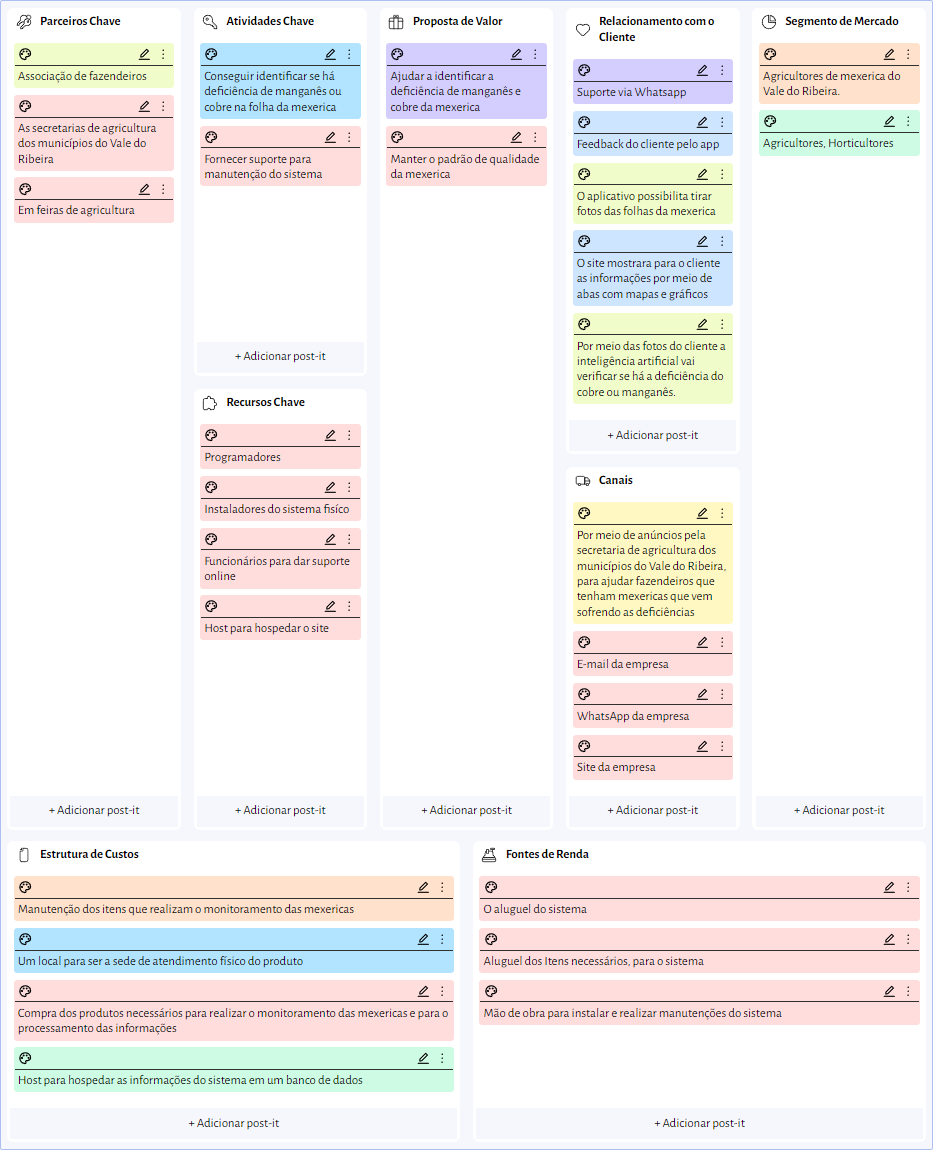
\includegraphics[width=0.8\linewidth]{Illustrations/canvas.png}
    \SourceOrNote{Autoria Própria (2025)}
    \end{figure}

    \section{APÊNDICE B — FLUXOGRAMA  DO MÉTODO DESENVOLVIDO}%
    \label{sect:apx-b1}

    \begin{figure}[H]
    \centering
    \caption{Figura B.1 -  Fluxograma do método de diagnóstico automatizado baseado em visão computacional}%
    \label{fig:fluxograma-metodo}
    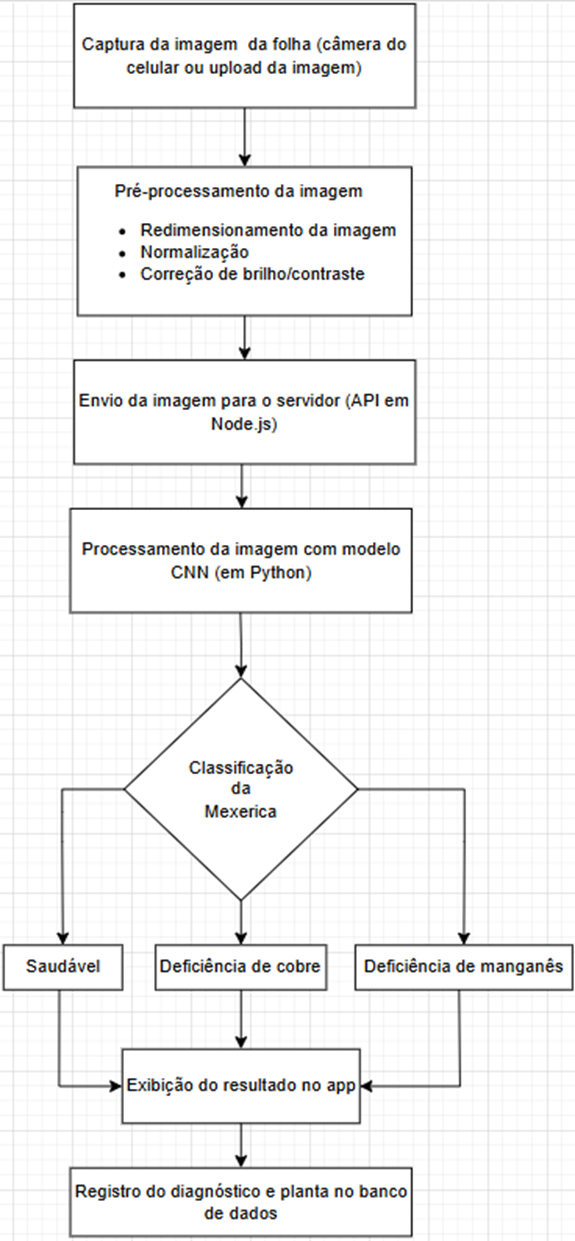
\includegraphics[width=0.4\linewidth]{Illustrations/fluxograma1.png}
    \SourceOrNote{Autoria Própria (2025)}
    \end{figure}
    
\end{Appendix}
    
    
    %% Índice remissivo
\printindex%
    

%% Fim do documento
\end{document}